\documentclass[aspectratio=169, compress]{beamer}

\usepackage[T1]{fontenc}
\usepackage[utf8]{inputenc}
\usepackage[english]{babel}
\usepackage{animate}
\usepackage{pgfplots}
\pgfplotsset{compat=newest}
\usepackage{booktabs}
\usepackage{siunitx}
\usepackage{subcaption}
\usepackage{tikz}
\usepackage{tikz-3dplot}
\usepackage{bm}
\usetikzlibrary{calc}
\usepackage{tikzpagenodes}
\usepackage{amsmath,amssymb,amsfonts, stmaryrd}
\usepackage{pgfplots}
\usetikzlibrary{shapes,arrows,decorations.pathmorphing,backgrounds,positioning,fit,matrix}
\usepackage{mathtools} %Fixes/improves amsmath
\usepackage{lipsum}
\pgfplotsset{compat=1.8}
\usepackage{graphics} % for pdf, bitmapped graphics files
\usepackage{epsfig} % for postscript graphics files
\usetikzlibrary{spy}
\usepackage[numbered,framed]{matlab-prettifier}
\usetikzlibrary{tikzmark}
\usetikzmarklibrary{listings}
\newcounter{tmkcount}
\usepackage{filecontents}

% Latin Modern
\usepackage{lmodern}
% Verdana font type
%\usepackage{verdana}
% Helvetica
%\usepackage{helvet}
% Times (text and math)
%\usepackage{newtx, newtxmath}
% Nice font combination
%\usepackage{mathptmx} % math
%\usepackage{sourcesanspro} % sans-serif
\usepackage{charter} % serif

\usetheme[department=space]{DTU}
%\useoutertheme[subsection=false]{miniframes}
%\useoutertheme{split}
\setbeamercovered{transparent}
%\setcounter{currentslide}{\the\beamer@slideinframe}

\title{Photogrammetry (30540)}
\subtitle{Feedback of assignments}
\author{\textbf{Instructor}: Daniel Olesen$^1$ Xiao Hu$^2$\\
	\textbf{TA}: Xiao Hu$^2$}
\institute{$^1$: Assistant Professor, Dept. of Geodesy\\ $2$: PhD student}
\date{\today}

\newcommand{\tabitem}{{\color{dtured}$\bullet$} }
\let\ph\mlplaceholder % shorter macro
\lstMakeShortInline"

\lstset{
  style              = Matlab-editor,
  basicstyle         = \mlttfamily,
  escapechar         = ",
  mlshowsectionrules = true,
}
\newcommand{\parallelsum}{\mathbin{\!/\mkern-5mu/\!}}


\begin{filecontents*}{q1.m}
%% Q1 
qhomo = [[3 4 1]; ...
     [4 6.5 0.5]; ...
     [5 2 0.1]; ...
     [10 100 20]; ...
     [0.1 0.2 100]]'; % homogeneous 
qinhomo = qhomo ./ qhomo(end,:);% inhomogeneous
\end{filecontents*}

\begin{filecontents*}{q2.m}
%% Q3
p1 = [1 2 1]';p2 = [5 3.5 1]';
l1 = cross(p1,p2);
%% Q4
scale = 1./norm(l1(1:2)); l1 = l1.*scale;
p3 = [7.5 3.6 1]';
dist = abs(p3'*l1);
%% Q5
l1 = [1 1 -1]'; l2 = [-1 3 -4]';
pinter = cross(l1,l2);
pinter = pinter ./ pinter(3);% to inhomogeneous
\end{filecontents*}

\begin{filecontents*}{q3.m}
%% Q8
A = [0.5 0.3 2; ...
     0.1 1.2 -2; ...
     0 0 1];  
pt1 = A*pt;
pt1 = pt1./pt1(3,:);
plot(pt(1,:), pt(2,:), 'LineWidth', 2);hold on;
plot(pt1(1,:), pt1(2,:),'r--');hold on;
\end{filecontents*}

\begin{filecontents*}{q4.m}
l1 = cross(q(:,1),q(:,2)); 
l2 = cross(q(:,3),q(:,4));
l3 = cross(q(:,1),q(:,4));
l4 = cross(q(:,2),q(:,3));% parallel lines
% vanishing points
p1 = cross(l1,l2);p1 = p1./p1(3);
p2 = cross(l3,l4);p2 = p2./p2(3);
% vanishing line
linf = cross(p1,p2);
linf = linf ./ linf(3);
% H
H = [1 0 0;0 1 0;linf(1) linf(2) linf(3)];
% warp
Iw = warpping(I,H);
\end{filecontents*}

\begin{filecontents*}{q5.m}
Q=Box3D;
plot3(Q(1,:),Q(2,:),Q(3,:),'.');
Qh = tohomogeneous(Q);
R = Rxyz(0.2, -0.3, 0.1);
t = [0.88;0.57;0.19];
f = 1000; cu = 300; cv = 200;
K = [f 0 cu;0 f cv;0 0 1];
P = K*[R t];
qc = P*Qh;% projection
q = qc ./ qc(3,:);% inhomogeneous
plot(q(1,:),q(2,:),'.')
\end{filecontents*}

\begin{filecontents*}{q6.m}
k1 = -5e-1;k2 = -3e-1;k3 = -5e-1;% radial
p1 = 0;p2 = 0;% tangent
qn = K\q;% normalized
x = qn(1,:); y = qn(2,:);
r = (x.^2+y.^2);
dradial = 1+r.*k1+r.^2.*k2+r.^3.*k3;
dtangentx = 2*p1.*x.*y + p2.*(r + 2.*x.^2);
dtangenty = p1.*(r + 2.*y.^2) + 2*p2.*x.*y;
% add distortions
qd(1,:) = x.*dradial + dtangentx;
qd(2,:) = y.*dradial + dtangenty;
qd(3,:) = ones(1,size(qn,2));
q1 = K*qd;
q1 = q1./q1(3,:);
hold on;
plot(q1(1,:),q1(2,:),'.')
\end{filecontents*}

\begin{filecontents*}{q7.m}
function Irec = undistortImg(I, K, k1, k2, k3, p1, p2)
	% Rectify image.
	[xx0,yy0] = meshgrid(1:size(I,2),1:size(I,1));
	xx0 = xx0(:)'; yy0 = yy0(:)';
	xx1 = (xx0 - K(1,3))./K(1,1); yy1 = (yy0 - K(2,3))./K(2,2);% normalized
	[xx,yy] = forward(xx1,yy1,k1,k2,k3,p1,p2);% projection and distortion
	% nearest interpolation
	xxf = xx.*K(1,1) + K(1,3); yyf = yy.*K(2,2) + K(2,3);
	xx = round(xxf); yy = round(yyf);
	% choose pixels in view
	valid = xx >= 1 & xx <= size(I,2) & yy >= 1 & yy <= size(I,1);
	% sub to index
	ind0 = sub2ind([size(I,1),size(I,2)], yy(valid), xx(valid));
	ind1 = sub2ind([size(I,1),size(I,2)], yy0(valid), xx0(valid));
	% assign value to rectified image
	Irec = uint8(zeros(m,n)); Irec(ind1) = I(ind0); 
end   
\end{filecontents*}

\begin{filecontents*}{q8.m}
function [xx,yy] = forward(xx,yy,k1,k2,k3,p1,p2)
% Apply distorsiton forward.
    r2 = xx.^2 + yy.^2;
    r4 = r2.*r2;
    r6 = r4.*r2;
    xy = xx.*yy;

    dradial = 1+r2.*k1+r4.*k2+r6.*k3;
    dtangentx = 2*p1.*xy + p2.*(r2 + 2.*xx.^2);
    dtangenty = p1.*(r2 + 2.*yy.^2) + 2*p2.*xy;

    xx = xx.*dradial + dtangentx;
    yy = yy.*dradial + dtangenty;
end    
\end{filecontents*}

\begin{filecontents*}{q9.m}
function F = DLT8pt(x1,x2)
%Implementation of 8 point algorithm for fundamental matrix estimation.
    if size(x1,1) ~= 3
        x1h = tohomo(x1);% to homogeneous
    end
    if size(x2,1) ~= 3
        x2h = tohomo(x2);
    end
    A = zeros(size(x1,2),9);
    for i = 1:size(x1,2)
        A(i,:) = kron(x1h(:,i)', x2h(:,i)');
    end
    [~,~,V] = svd(A);
    F = V(:,end);
    F = F([1 4 7;2 5 8;3 6 9]);
    F = F./F(3,3);
end
\end{filecontents*}

\begin{filecontents*}{q10.m}
function P = triangulationSVD(x1,P1,x2,P2)
%Implementation of SVD triangulation method.
    A(1,:) = (x1(1).*P1(3,:) - P1(1,:));
    A(2,:) = (x1(2).*P1(3,:) - P1(2,:));
    A(3,:) = (x2(1).*P2(3,:) - P2(1,:));
    A(4,:) = (x2(2).*P2(3,:) - P2(2,:));
    [~,~,V] = svd(A);
    P = V(:,end);
    P = P(1:3)./P(end);
end
\end{filecontents*}

\begin{filecontents*}{q11.m}
function xyz = stereoTriangulate(disp, f, cx, cy, b,id)
% function xyz = stereoTriangulate(disp, f, cx, cy, b,id)
    z = f * b ./ disp(id);
    [yy,xx] = find(id);
    x = (xx - cx).*z / f;
    y = (yy - cy).*z / f;
    xyz = [x y z];
end
\end{filecontents*}


\begin{filecontents*}{q12.m}
%% Harris corner detector
Ix = edge(im,'Sobel',[],'horizontal'); Iy = edge(im,'Sobel',[],'vertical');% gradient
figure; subplot(1,2,1);imshow(Ix); subplot(1,2,2);imshow(Iy);% plot
% Ixx, Iyy, Ixy
Ixx = Ix.*Ix; Iyy = Iy.*Iy; Ixy = Ix.*Iy;
% gaussian kernel
g = fspecial('gaussian', 3, 1);
% smoothing
Ixx = imfilter(Ixx,g,'replicate'); Iyy = imfilter(Iyy,g,'replicate'); 
Ixy = imfilter(Ixy,g,'replicate');
% response map
C = Ixx.*Iyy - Ixy.^2 - 0.04.*(Ixx+Iyy).^2;
% thresholding
threshold = 0.3*max(C(:)); C(C(:)<threshold) = 0;
figure; imshow(C);
% nonmaxima suppression
[row,col] = nonmaxsuppts(C,'radius', 2, 'N', 1000);
% plot
figure; img=imshow(imColor),title('my-Harris'); hold on
plot(col,row, 'ro','MarkerSize',10),
\end{filecontents*}

\begin{filecontents*}{q13.m}
	number = size(ph,2); % total points
	sigma =0.1;   %threshold
	best_inlier_cnt = 0; best_line = [];% save best result
	for i=1:200
		% random sample
   		idx = randperm(number,2);
 	  	prand1 = ph(:, idx(1)); prand2 = ph(:, idx(2));
		% model estimation
		line=cross(prand1,prand2);  		
  		% compute consensus
  		consensus=abs(line' * ph )./ sqrt(line(1)^2+line(2)^2);
		% classifier inliers
		inlier=consensus(consensus<0.1);
		% check if better
  		if best_inlier_cnt < length(inlier)
    		best_inlier_cnt = length(inlier); best_line = line;
		end
	end
  	params=best_line;
\end{filecontents*}

\begin{document}
	\frame{
		\maketitle
	}	
	
	\section{Camera Model \& Homogenous Coordinates}
	\subsection{Homogeneous Coordinates}
	\begin{frame}[fragile]
		\frametitle{Q1, Q2: From homogeneous coordinates to inhomogeneous coordinates} 
		\begin{columns}
			\column[c]{.5\textwidth}		
			dividing with the last element:
			\begin{align*}
			\underbrace{
			\left[
			\begin{matrix}
			x \\ y \\ \vdots \\ w
			\end{matrix}\right]}_{homogeneous} \to \underbrace{
			\left[
			\begin{matrix}
			x/w \\ y/w \\ \vdots
			\end{matrix}\right]}_{inhomogeneous}
			\end{align*}
			\column[c]{.5\textwidth}
		 \lstinputlisting[basicstyle=\small, caption = {code},language=Matlab]{q1.m}
			\end{columns}
\end{frame}

	\begin{frame}[fragile]
		\frametitle{Q3, Q4, Q5: find line, point-to-line distance, and intersected point \\ using homogeneous coordinates}
		\begin{columns}
			\column[c]{.5\textwidth}		
			\begin{itemize}
			\item line $\mathbf{l}$ which passes two 2D points $\mathbf{p}_1$, $\mathbf{p}_2$: $\mathbf{l}=\text{cross}(\mathbf{p}_1,\mathbf{p}_2)$
			\item point $\mathbf{p}$ to line $\mathbf{l}$ distance: $d=\frac{\mathbf{p}^T\mathbf{l}}{\sqrt{\mathbf{l}(1)^2+\mathbf{l}(2)^2}}$
			\item the intersection $\mathbf{p}$ of two lines $\mathbf{l}_1, \mathbf{l}_2$: $\mathbf{p}=\text{cross}(\mathbf{l}_1,\mathbf{l}_2)$
			\end{itemize}
			\column[c]{.5\textwidth}
		 \lstinputlisting[basicstyle=\small, caption = {code},language=Matlab]{q2.m}
			\end{columns}
\end{frame}

	
	\frame{
		\frametitle{Q6,Q7,Q8: Euclidean, Similarity, Affine Transformation} 
		\begin{columns}
		\column[c]{.5\textwidth}	
		\begin{figure}
			\centering
			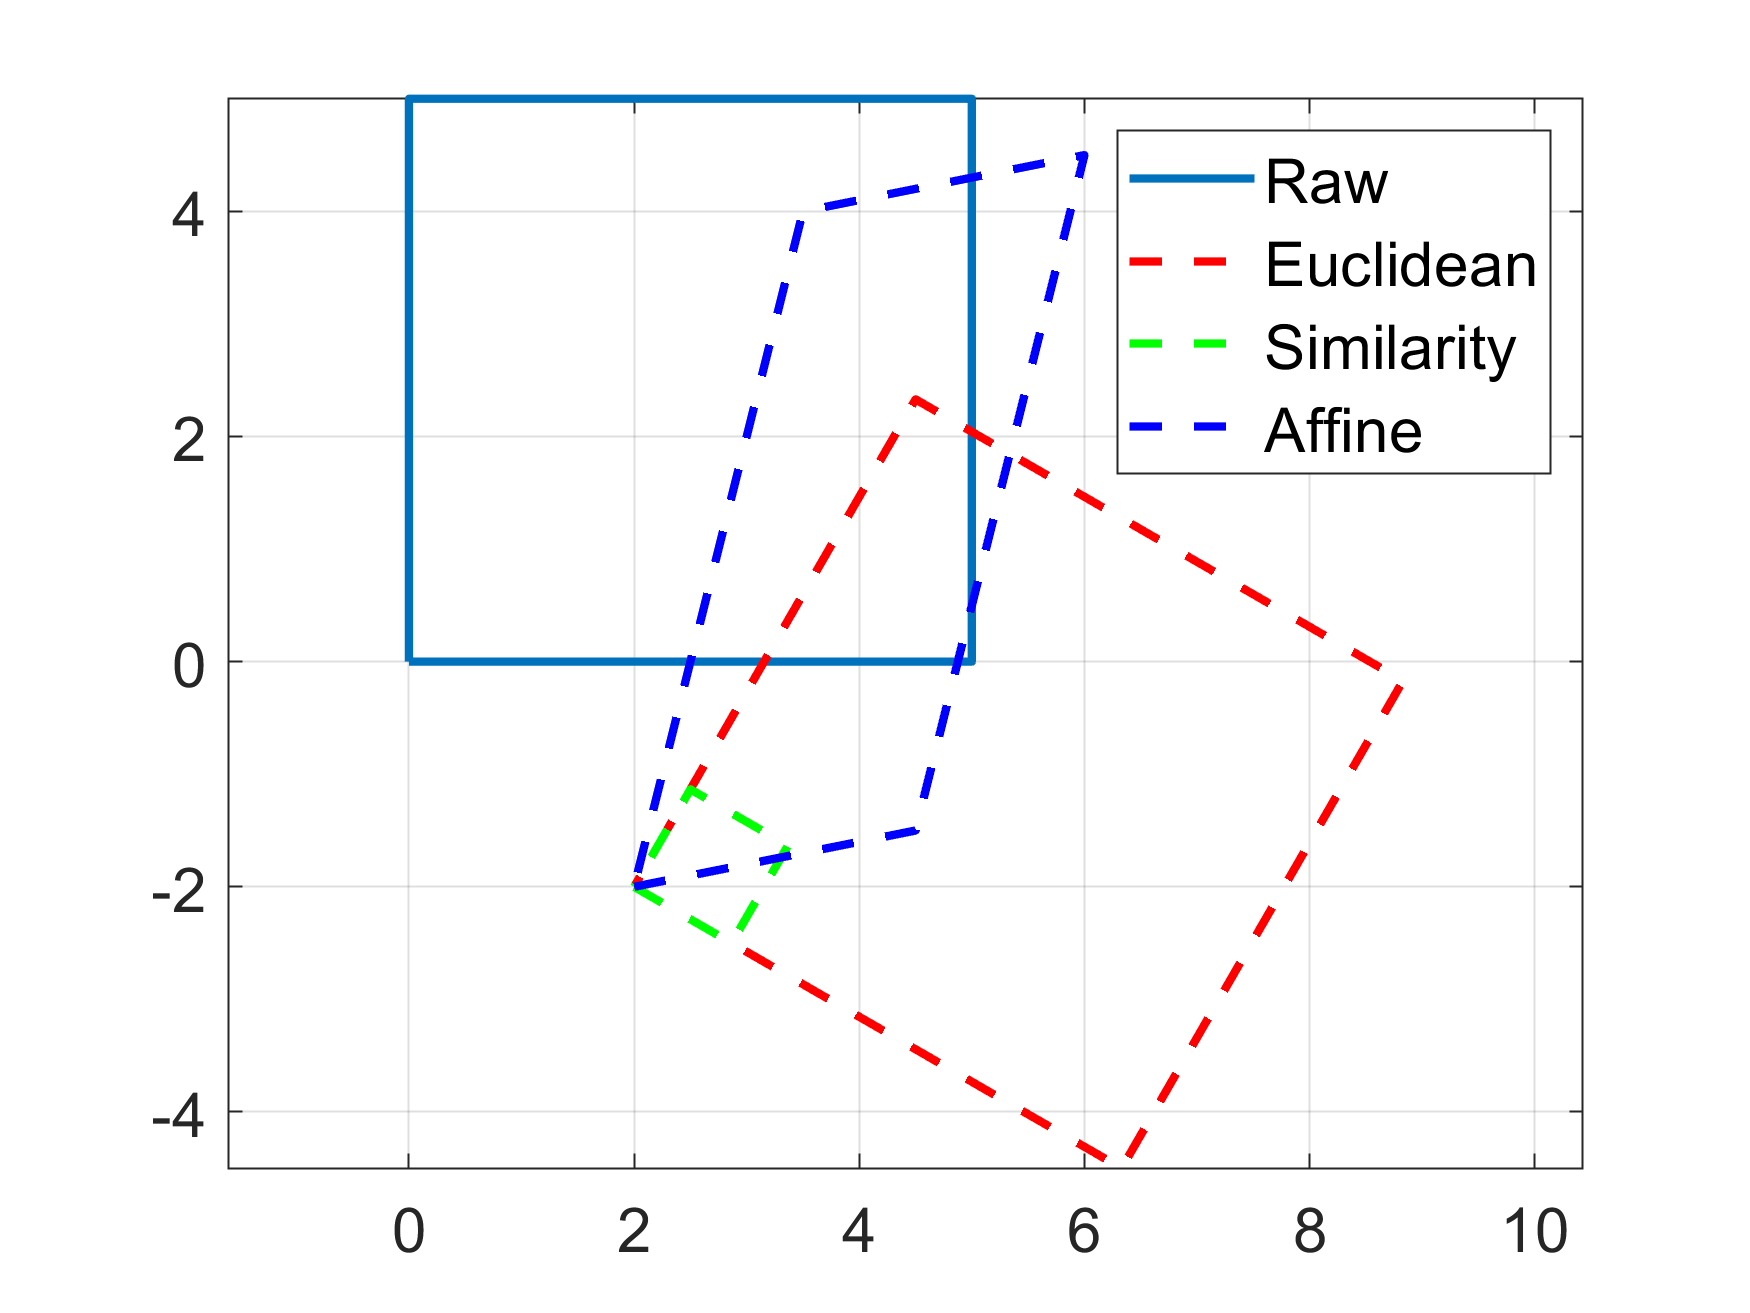
\includegraphics[width=1\textwidth]{figures/ex1_2.png}
		\end{figure}		
		\column[c]{.5\textwidth}
		 \lstinputlisting[basicstyle=\small, caption = {code},language=Matlab]{q3.m}
		\end{columns}
	}	
	
	\frame{
		\frametitle{Q6,Q7,Q8: Invariant properties} 
		\begin{columns}
		\column[c]{.5\textwidth}	
		\begin{figure}
			\centering
			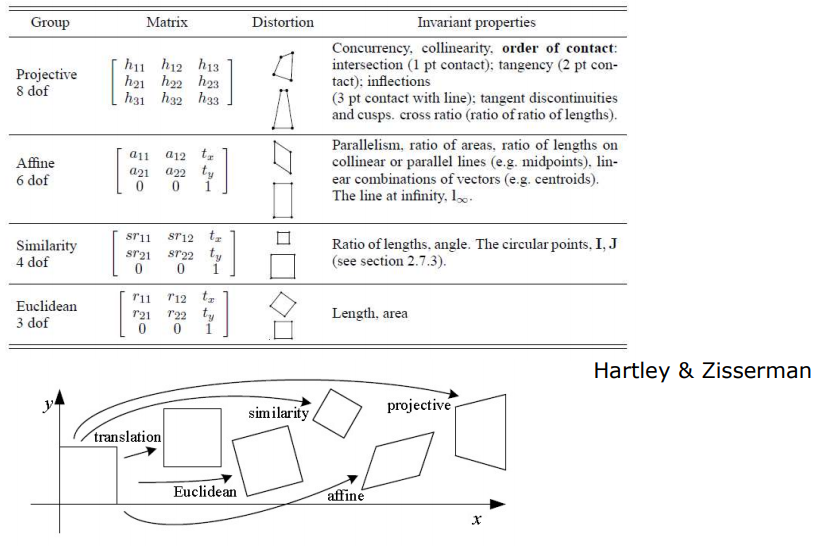
\includegraphics[width=1.3\textwidth]{figures/ex1_1.png}
		\end{figure}		
		\column[c]{.5\textwidth}
		\begin{figure}
			\centering
			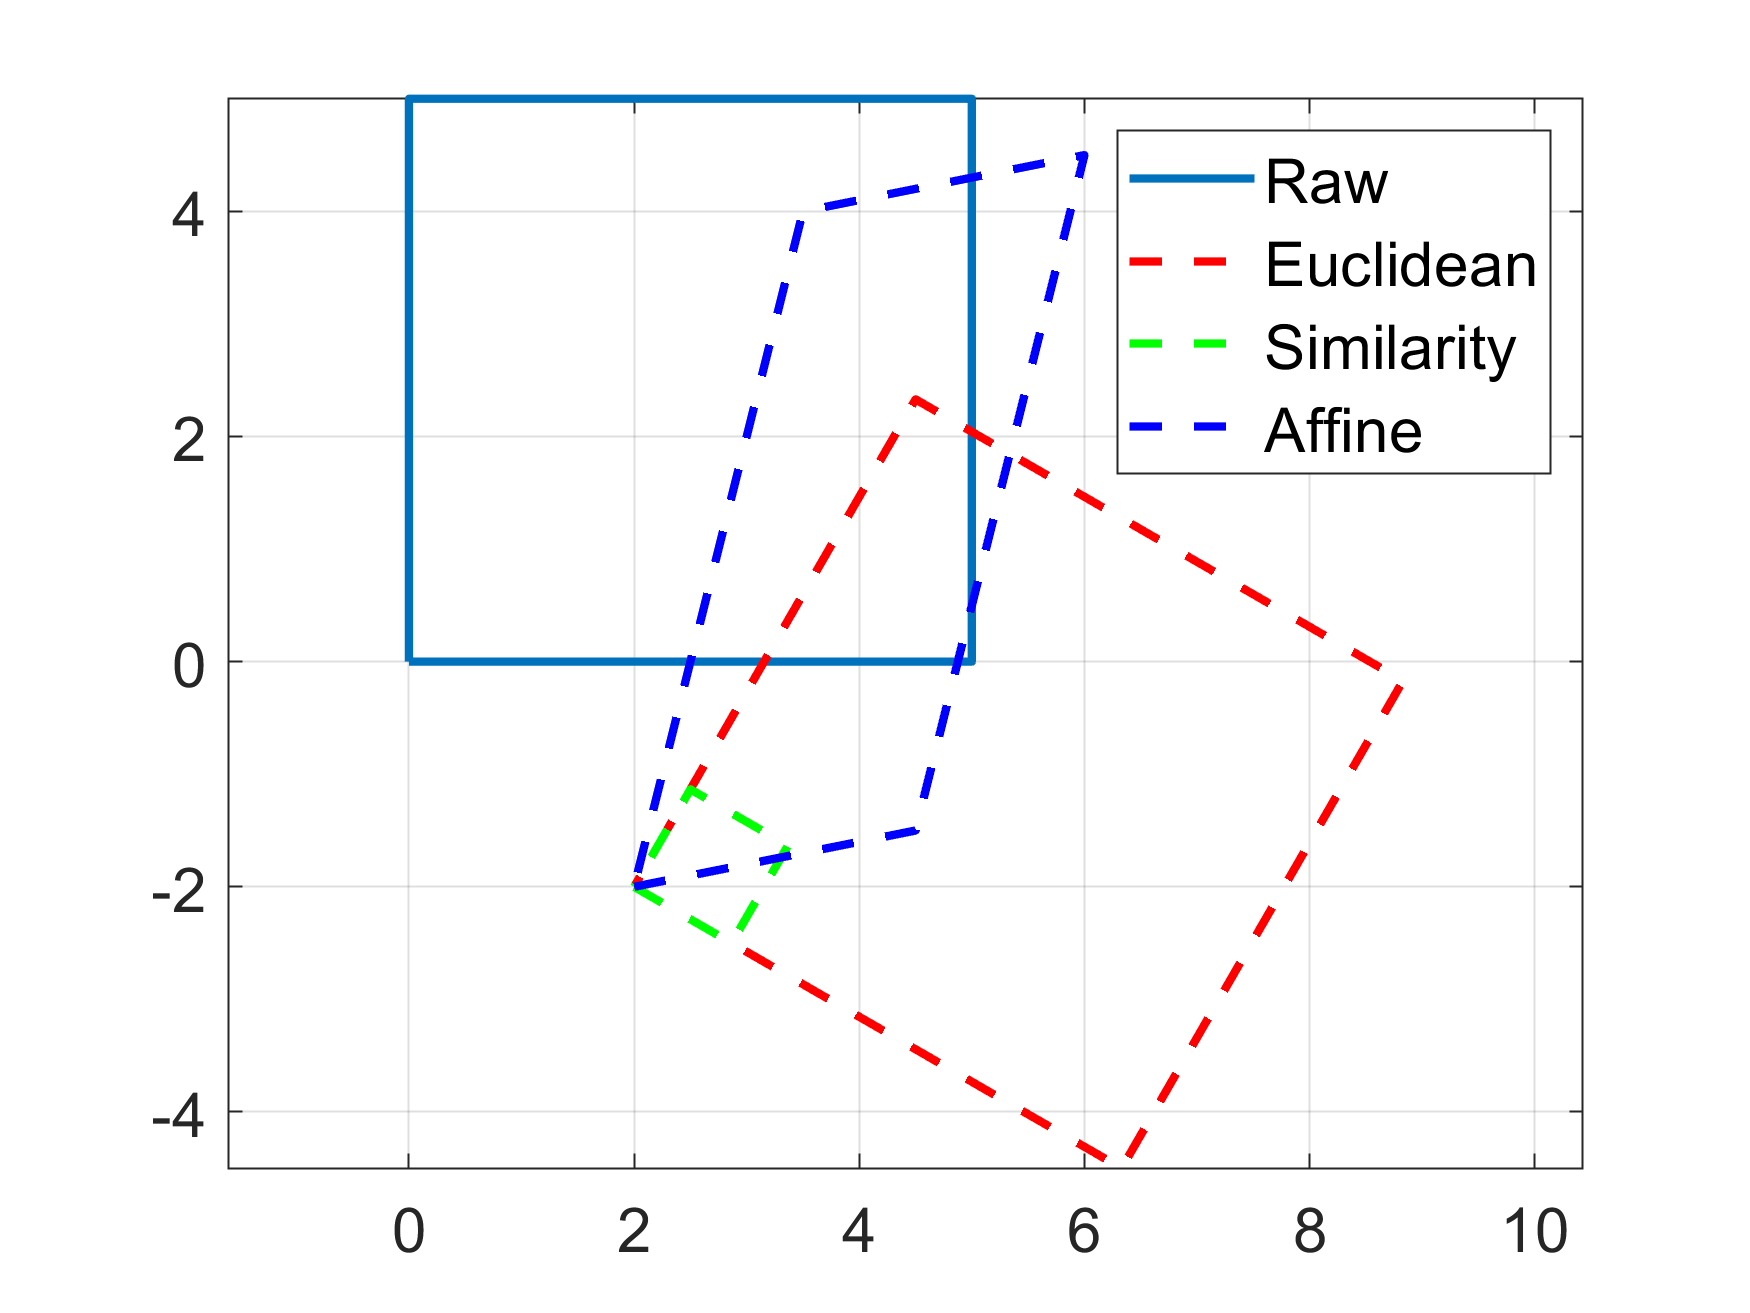
\includegraphics[width=1\textwidth]{figures/ex1_2.png}
		\end{figure}		
		\end{columns}
	}	
	
	\frame{
		\frametitle{Q9: Inverse Perspective Mapping} 
		\begin{columns}
		\column[c]{.5\textwidth}	
		\begin{itemize}
		\item find parallel lines $\mathbf{l}_1 \parallelsum \mathbf{l}_2$, $\mathbf{l}_3 \parallelsum \mathbf{l}_4$
		\item find vanishing points $\mathbf{p}_1=\text{cross}(\mathbf{l}_1,\mathbf{l}_2)$, $\mathbf{p}_2=\text{cross}(\mathbf{l}_3,\mathbf{l}_4)$
		\item vanishing line $\mathbf{l}_{inf}=\text{cross}(\mathbf{p}_1,\mathbf{p}_2)$
		\item $\mathbf{H}=\left[
		\begin{matrix}
		1 & 0 & 0 \\
		0 & 1 & 0 \\
		\mathbf{l}_{inf}(1) & \mathbf{l}_{inf}(2) & \mathbf{l}_{inf}(3)
		\end{matrix}				
		\right]$
		\item Warp
		\end{itemize}
		\column[c]{.5\textwidth}
		\vspace{-1cm}
		\lstinputlisting[basicstyle=\small, caption = {code},language=Matlab]{q4.m}
		\end{columns}
	}	


	\section{Intrinsics, Extrinsics \& P3P}	
	\frame{
		\frametitle{Q1: Intrinsics, Extrinsics} 
		\begin{columns}
		\column[c]{.5\textwidth}	
		\begin{itemize}
		\item Intrinsics $\mathbf{K}=\left[
		\begin{matrix}
		f_x & 0 & p_x \\
		0 & f_y & p_y \\
		0 & 0 & 1
		\end{matrix}				
		\right]$
		\item Projective matrix $\mathbf{P}=\mathbf{K}(\mathbf{R}\ \mathbf{t})$
		\item Projection $\mathbf{x}=\mathbf{P}\mathbf{X}$
		\item To inhomogeneous coordinate
		\end{itemize}
		\column[c]{.4\textwidth}
		\vspace{-1cm}
		\lstinputlisting[basicstyle=\small, caption = {code},language=Matlab]{q5.m}
		\end{columns}
	}	
	\frame{
		\frametitle{Q2: radial, tangent distortions} 
		\begin{columns}
		\column[c]{.4\textwidth}	
		\begin{itemize}
		\item apply extrinsics $ \mathbf{x}' = \left(\mathbf{R} | \mathbf{t}\right) \mathbf{X} $
		\item to inhomogeneous coordinates
$
\mathbf{x}''(1)=\frac{\mathbf{x}'(1)}{\mathbf{x}'(3)},\ \mathbf{x}''(2)=\frac{\mathbf{x}'(2)}{\mathbf{x}'(3)}
$
		\item apply radial distortion model
\begin{align*}
r^2 &= \mathbf{x}''(1)^2+\mathbf{x}''(2)^2 \\
\mathbf{x}''(1) &= \mathbf{x}''(1)(1+a_1r^2+a_2r^4+a_3r^6) \\
\mathbf{x}''(2) &= \mathbf{x}''(2)(1+a_1r^2+a_2r^4+a_3r^6)
\end{align*}
		\item multiply $\mathbf{K}$: $
\mathbf{x}''' = \mathbf{K}\left[
\begin{matrix}
\mathbf{x}''(1) \\ \mathbf{x}''(2) \\ 1
\end{matrix}
\right]$
\end{itemize}
		\column[c]{.6\textwidth}
		\vspace{-1cm}
		\lstinputlisting[basicstyle=\small, caption = {code},language=Matlab]{q6.m}
		\end{columns}
	}	
	
\frame{
		\frametitle{Q2: radial, tangent distortions} 
		\begin{columns}
		\column[c]{1\textwidth}	
		\begin{figure}
			\centering
			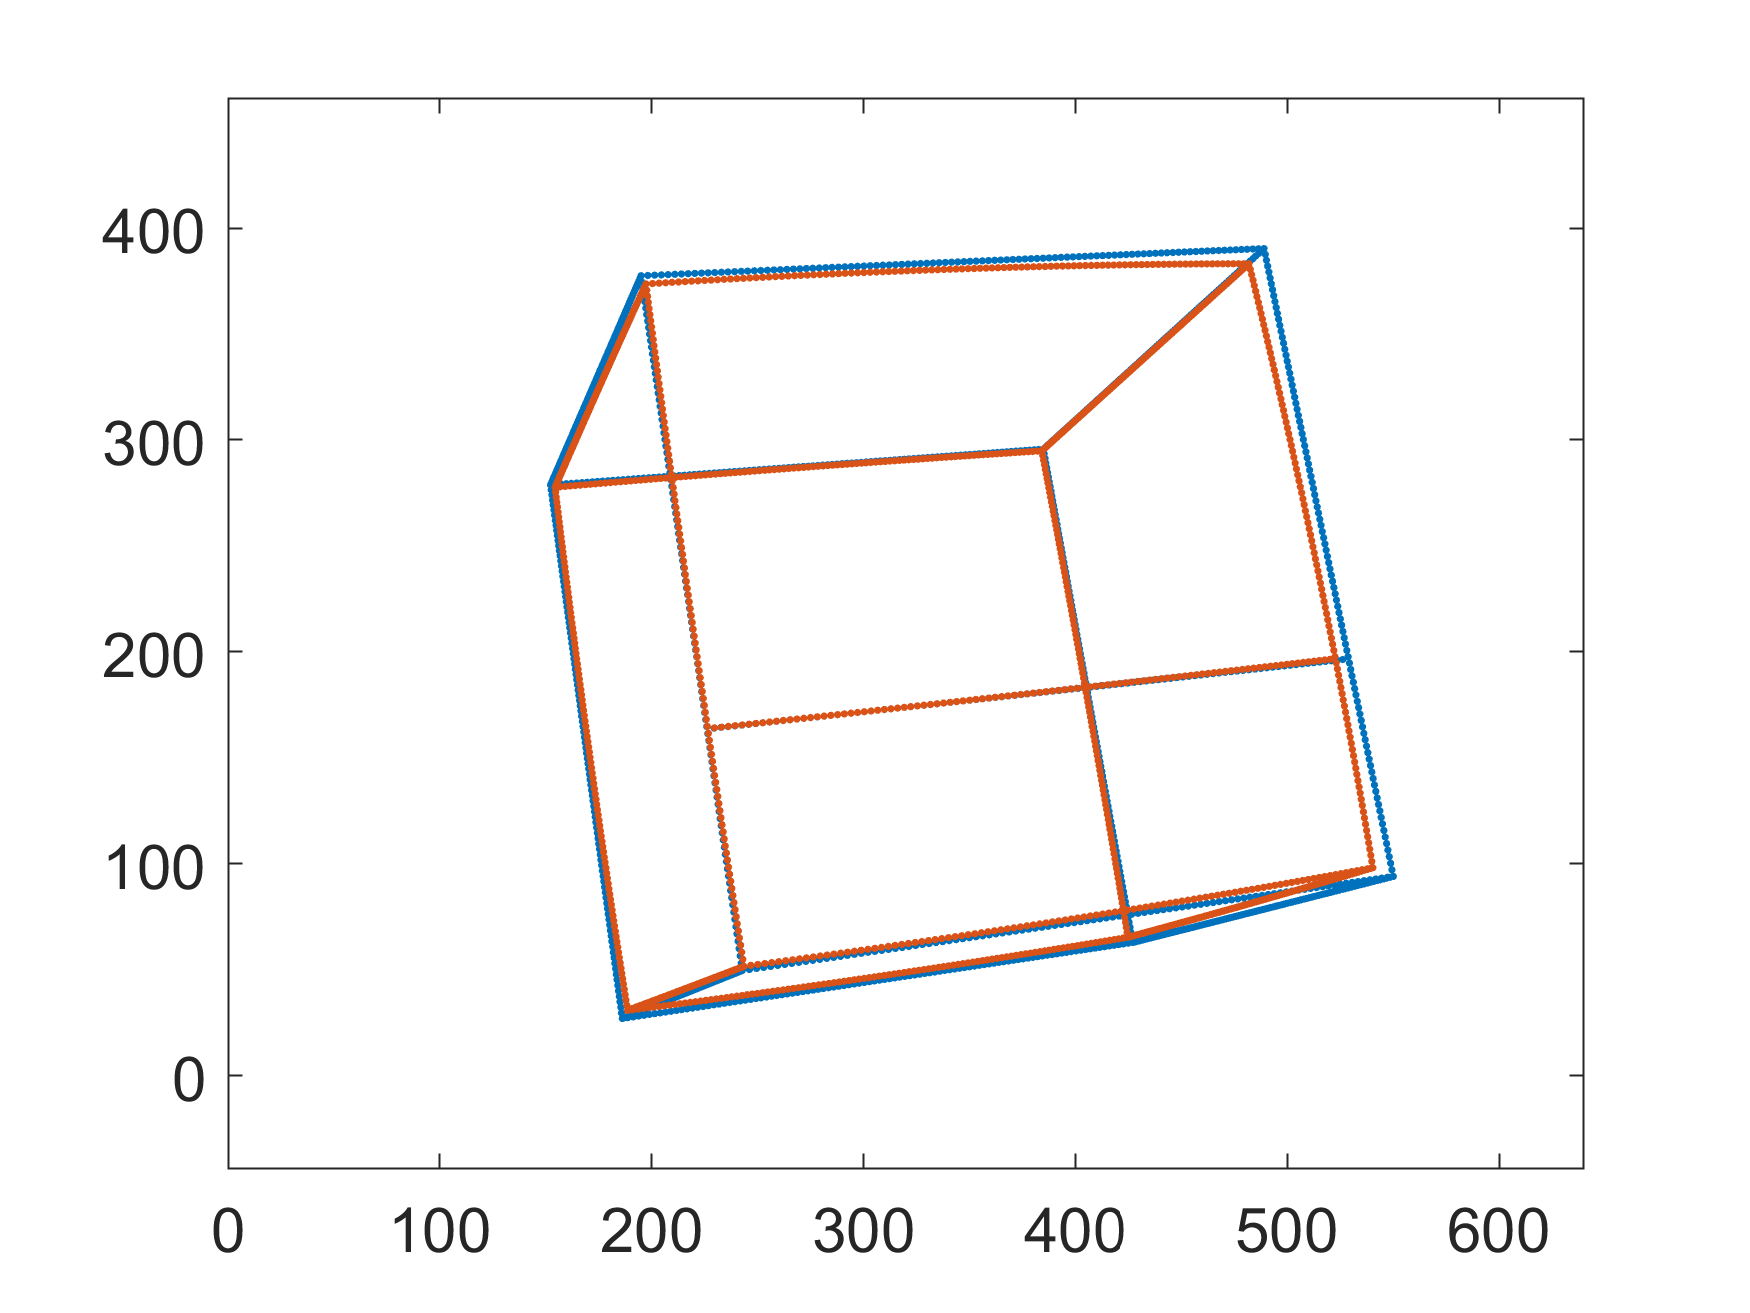
\includegraphics[width=0.5\textwidth]{figures/ex2_1.png}
		\end{figure}	
		\end{columns}
	}		
	
\frame{
		\frametitle{Q4: rectification} 
		\vspace{-0.7cm}
		\lstinputlisting[basicstyle=\small, caption = {code},language=Matlab]{q7.m}
	}
	
\frame{
		\frametitle{Q4: rectification} 
		\vspace{-1cm}
		\lstinputlisting[basicstyle=\small, caption = {code},language=Matlab]{q8.m}
	}
	
\frame{
		\frametitle{Q5: Perspective $3$ Point} 
		Solution has been uploaded. See \cite{c1} for the explanations for those mathematical equations.
	}	
	
	
		
	\section{Epipolar Geometry \& Triangulation}
	\frame{
		\frametitle{Q1: Fundamental Matrix using $8$ point algorithm} 
		\vspace{-0.5cm}
		\lstinputlisting[basicstyle=\fontsize{9}{11}\ttfamily, caption = {code},language=Matlab]{q9.m}
	}
	\frame{
		\frametitle{Q2: Triangulation} 
\begin{columns}
		\column[c]{.5\textwidth}	
\begin{align*}
&\left[\begin{matrix}
x_1(1) \\ x_1(2) \\ 1
\end{matrix}\right]=\left[\begin{matrix}
\frac{\mathbf{P}_1(1,:)\mathbf{X}}{\mathbf{P}_1(3,:)\mathbf{X}} \\ 
\frac{\mathbf{P}_1(2,:)\mathbf{X}}{\mathbf{P}_1(3,:)\mathbf{X}} \\ 
1
\end{matrix}\right] \Rightarrow \\
&\left[\begin{matrix}
\mathbf{P}_1(3,:)x_1(1)-\mathbf{P}_1(1,:) \\
\mathbf{P}_1(3,:)x_1(2)-\mathbf{P}_1(2,:)
\end{matrix}\right]\mathbf{X} = 0
\end{align*}		
One projection contributes to two equations, we need two points for solving $\mathbf{X}$:
\begin{align*}
&\left[\begin{matrix}
\mathbf{P}_1(3,:)x_1(1)-\mathbf{P}_1(1,:) \\
\mathbf{P}_1(3,:)x_1(2)-\mathbf{P}_1(2,:) \\
\mathbf{P}_2(3,:)x_2(1)-\mathbf{P}_2(1,:) \\
\mathbf{P}_2(3,:)x_2(2)-\mathbf{P}_2(2,:) \\
\end{matrix}\right]\mathbf{X} = 0
\end{align*}
		\column[c]{.5\textwidth}
		\vspace{-1cm}
		\lstinputlisting[basicstyle=\fontsize{8}{10}\ttfamily, caption = {code},language=Matlab]{q10.m}
		\end{columns}
	}
	\frame{
	\frametitle{Q4: Triangulation with stereo disparity map} 
	\begin{columns}
		\column[c]{.5\textwidth}	
The equations for triangulate points using disparity:
\begin{align*}
Z &= \frac{f*b}{d} \\
X &= \frac{(x-p_x)Z}{f} \\ 
Y &= \frac{(y-p_y)Z}{f}
\end{align*}
here, $p_x,p_y$ are the coordinates of the principal point, $f$ is the focus length, $b$ is the baseline.
	\column[c]{.5\textwidth}
		\vspace{-1cm}
		\lstinputlisting[basicstyle=\fontsize{8}{10}\ttfamily, caption = {code},language=Matlab]{q11.m}
		\end{columns}
	}
	

\section{Feature Detection \& Outlier rejection}
	\frame{
		\frametitle{Q1: Harris Corner Detector} 
		\vspace{-0.7cm}
		\lstinputlisting[basicstyle=\fontsize{8}{10}\ttfamily, caption = {code},language=Matlab]{q12.m}
	}
	\frame{
	\frametitle{Q2: RANSAC} 
		\vspace{-1cm}
		\lstinputlisting[basicstyle=\fontsize{8}{10}\ttfamily, caption = {code},language=Matlab]{q13.m}
	}
	
	\begin{thebibliography}{00}
	\bibitem{c1} Haralick B M, Lee C N, Ottenberg K, et al. Review and analysis of solutions of the three point perspective pose estimation problem[J]. International journal of computer vision, 1994, 13(3): 331-356..
	\end{thebibliography}	
	
\end{document}
